\part{Une nouvelle voie à définir pour Time Machine}

%===RETOUR SUR LE STAGE (CLARIFIER OU PLACER LA FEUILLE DE ROUTE)
\chapter{Stagiaire au sein du projet Time Machine}

Nous avons été engagée en tant que stagiaire au sein du \gls{dhlab} de l'\gls{epfl}, du 15 avril au 31 août 2019. Nous avons pris une part active dans l'élaboration de la future feuille de route du projet Time Machine.

\section{État des lieux avant le commencement du stage}
Lorsque nous avons commencé notre stage, Time Machine venait tout juste de recevoir le million d'euros de l'\gls{ue} pour démontrer la faisabilité du projet et tenter de remporter un milliard. Cette période appelée à se dérouler du 1er mars 2019 au 29 février 2020 est appelée \gls{csa} par l'\gls{ue}, et implique la collaboration des 32 partenaires du projet dans l'élaboration de solutions. Dans la proposition initialement soumise à l'\gls{ue}, quatre piliers, \textit{PILLARs}, correspondant à des thématiques particulières et devant proposer chacun une feuille de route détaillée contenant des solutions concrètes ont été identifiés et les responsabilités de chacun d'eux réparties parmi autant de groupes de travail composés de membres du consortium. 

En plus de ces différents piliers amenés à durer au-delà de la phase du \gls{csa}, différents \gls{wp} visent à accompagner la mise en place du projet durant cette année charnière. La temporalité des actions à mener est également préalablement définie au même titre que les interactions entre les différentes tâches composant chaque pilier, et les interactions entre les différents piliers. 

La liste des activités conduites durant la période du \gls{csa} peut se résumer ainsi :

\begin{enumerate}
\item \textit{WP 1: Project Management}
\item \textit{PILLAR 1: Science and Innovation}

Ayant pour objectif de proposer les différentes thématiques de recherches nécessaires au fonctionnement des futurs processus de l'infrastructure Time Machine.
\item \textit{PILLAR 2: Time Machine Operations}

Ayant pour objectif de mettre en place le projet, de définir son fonctionnement tant au niveau organisationnel que technologique.
\item \textit{PILLAR 3: Exploitation Avenues}

Ayant pour objectif de définir quels produits et services pourront être construits avec les données du projet et comment mettre en place la collaboration avec ses futurs utilisateurs.
\item \textit{PILLAR 4: Innovation and Outreach}

Ayant pour objectif de garantir la création d'une structure suffisamment flexible pour évoluer fortement en fonction des développements technologiques et demeurer suffisamment souple pour ne pas freiner l'innovation.
\item \textit{WP 6: Governance scheme}

Ayant pour objectif de mettre en place la gouvernance de Time Machine.
\item \textit{WP7: Dissemination and Promotion}

Ayant pour objectif la communication et valorisation du projet Time Machine.
\item \textit{WP8: Overall Time Machine Strategy and Implementation Plan}

Ayant pour objectif de garantir la cohérence globale et le développement futur de Time Machine.
\end{enumerate}


Certains groupes de travail doivent proposer des solutions plus tôt, afin que d'autres puissent bâtir leurs propositions en tenant compte des objectifs énoncés, c'est notamment le cas pour les \textit{PILLARs} 1, 2 et 3. 

Notre maître de stage, le Professeur Frédéric Kaplan, est chargé de la gestion du projet durant cette période du \gls{csa}.

Un consultant externe, déjà engagé pour la proposition initiale, se charge de superviser les différentes activités et propositions et offre une vision plus stratégique, nécessaire au bon développement du projet

Un coordinateur de projet a également été engagé pour la durée du \gls{csa}, chargé de mettre en place les outils collaboratifs nécessaires à des groupes de travail répartis entre plusieurs territoires et de professionnaliser les pratiques de Time Machine, en prenant en charge le management des risques et en proposant une supervision globale du projet. Les activités du chef de projet forment un \gls{wp} spécifique au temps du \gls{csa}.

Un comité exécutif réunissant les responsables des différents \textit{PILLARs}, le chef de projet, le consultant et le coordinateur se réunit virtuellement chaque semaine, afin de garantir un niveau d'échanges minimal entre les différents participants et pour faire face aux inévitables enjeux posés par un projet d'une telle envergure. Nous serons amenée à en faire partie durant toute la durée de notre stage.

\begin{figure}[H]% force à placer l'image au sein de notre balise figure
\centering
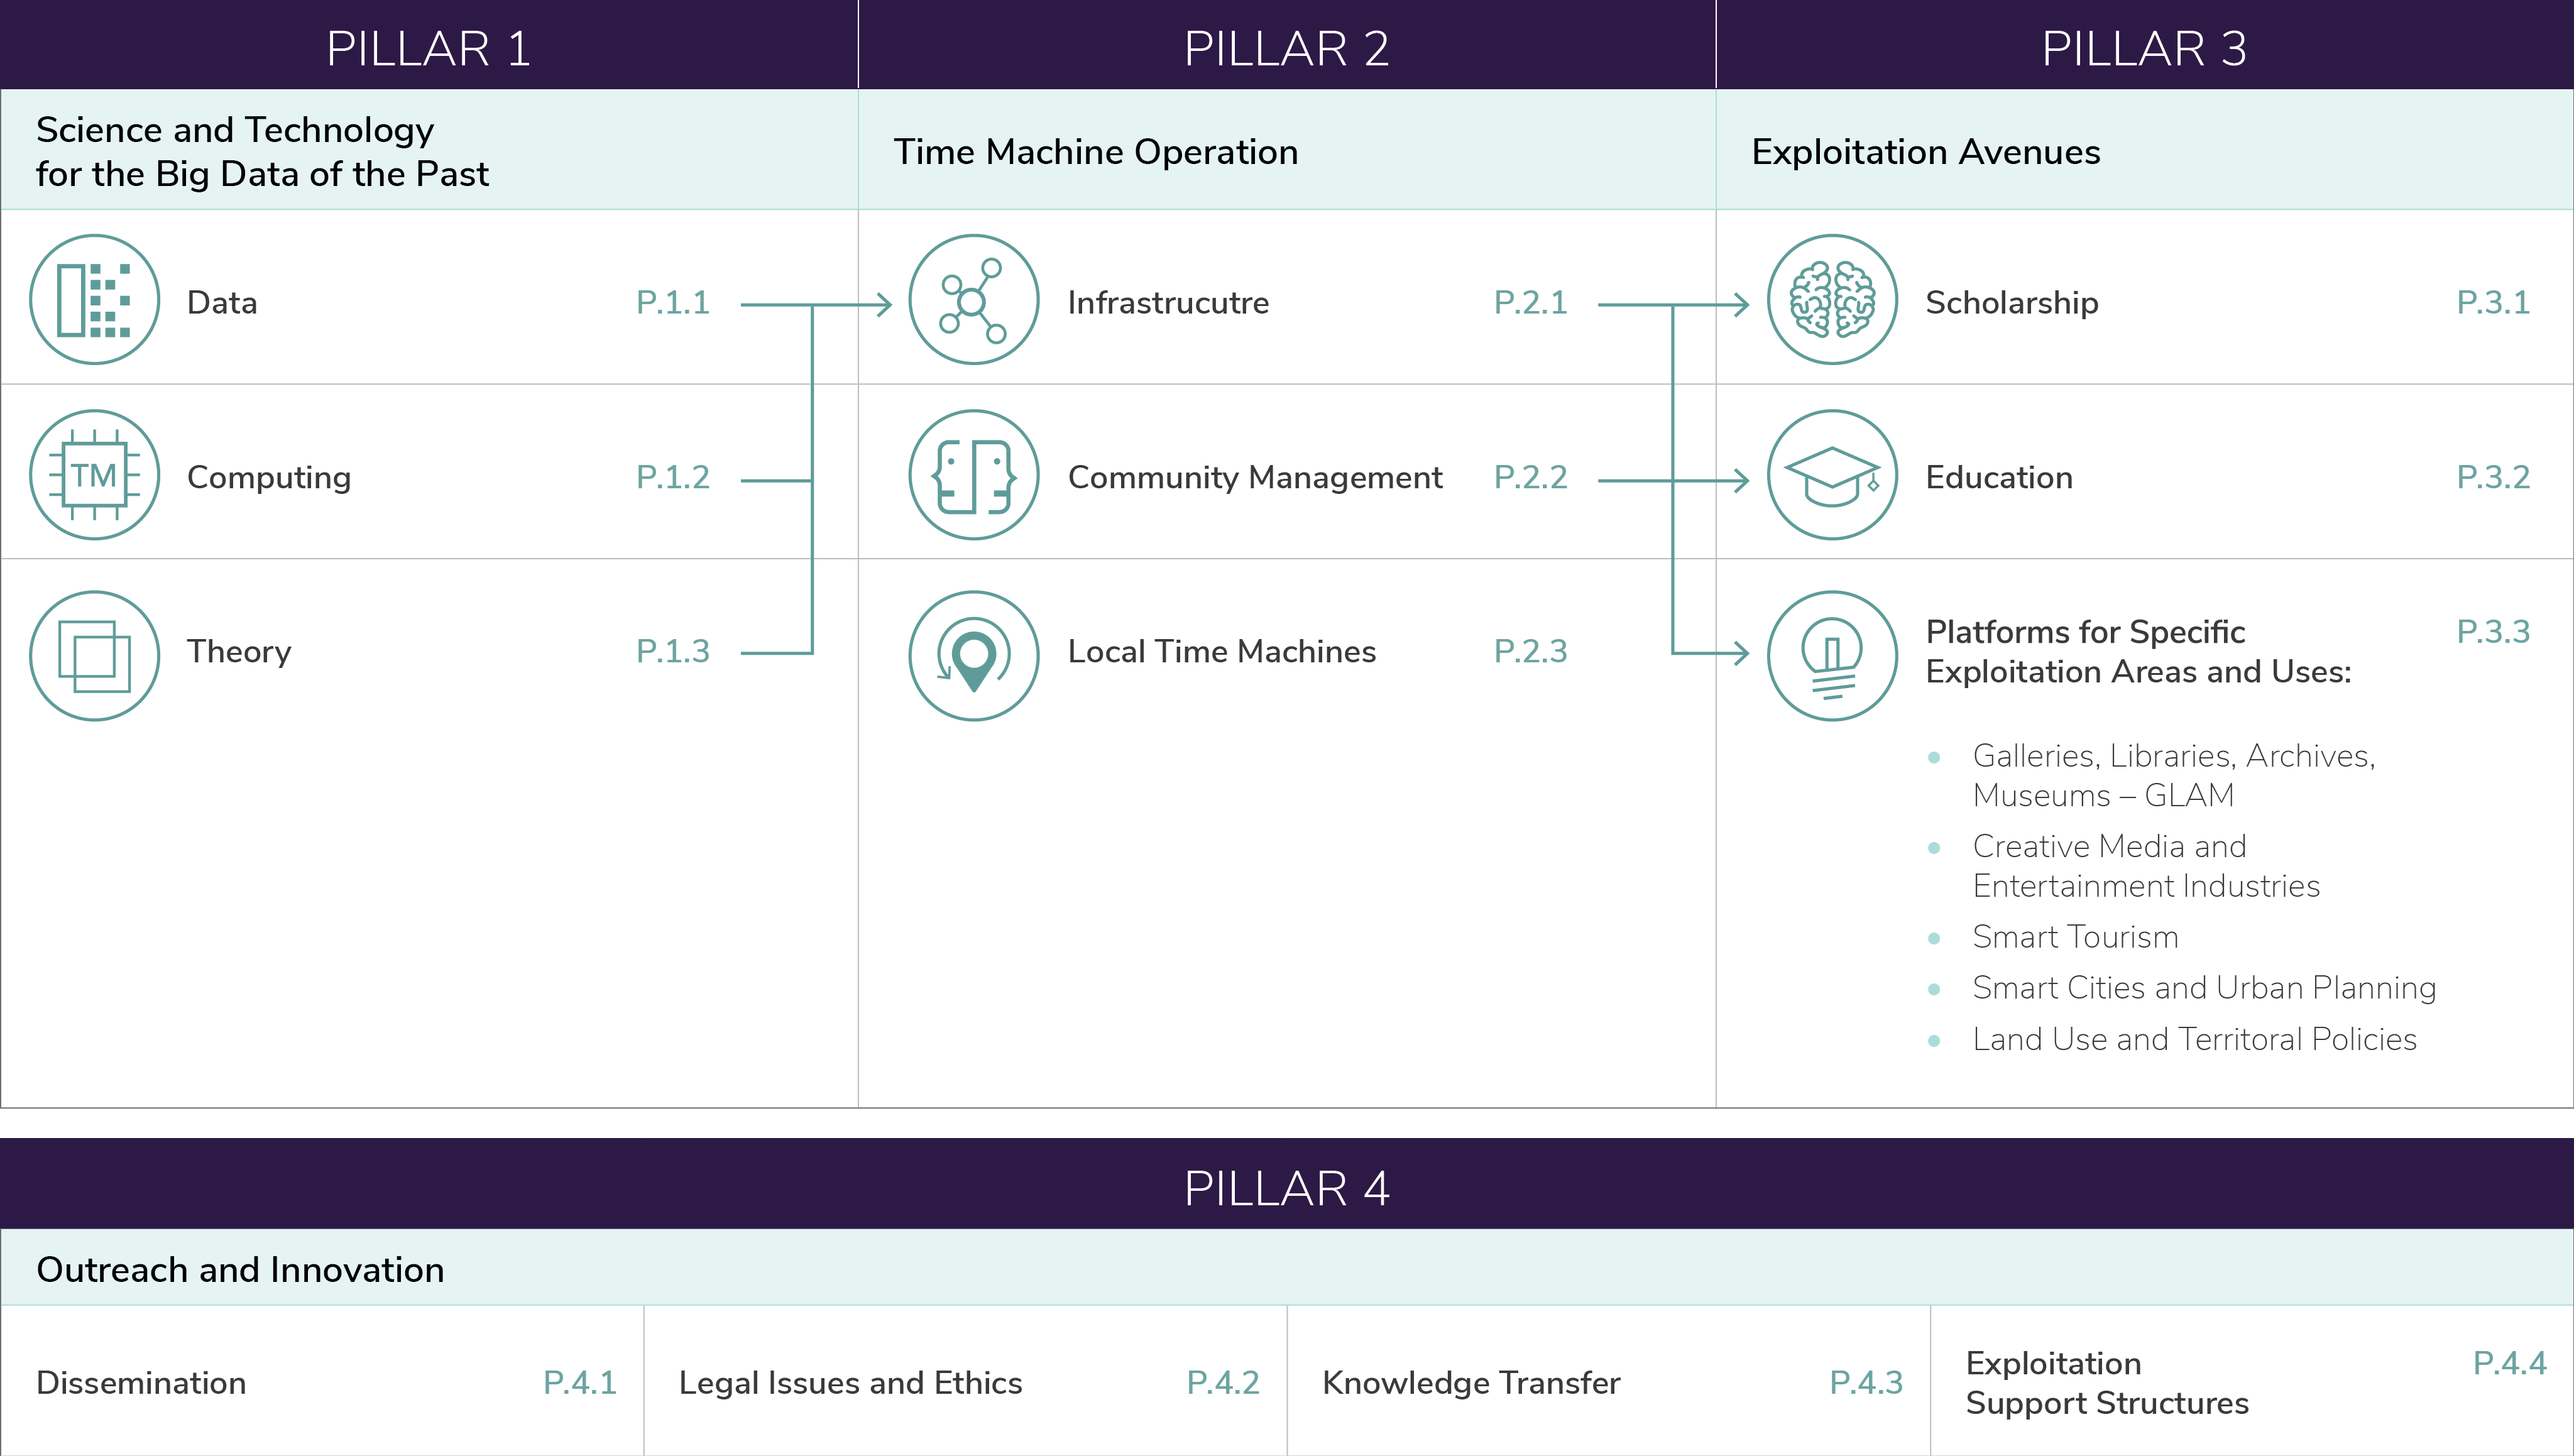
\includegraphics[width=15cm]{pillar_org.png}
\caption{Organisation et interactions des premiers \textit{PILLAR}s \textit{© Copyright 2019 Time Machine}}
\end{figure}

Cette période du \gls{csa} est également rythmée par différentes conférences\footnote{Nous participerons à la deuxième conférence, réunissant les groupes de travail des différents \textit{PILLAR}, les 9-10 mai à Amsterdam}, visant à réunir les partenaires afin de faciliter la collaboration au sein des membres d'un même PILLAR ou \gls{wp}, de faire connaître le projet et d'inviter les membres croissants à collaborer à ce processus décisionnel. En effet, le réseau Time Machine grandit en parallèle de la période du \gls{csa} et bien que les nouveaux membres ne soient pas liés contractuellement à l'élaboration du projet, ni rémunérés par l'\gls{ue}, les échanges sont fortement encouragés. Lors de la conférence d'Amsterdam des 9 et 10 mai 2019, plus d'une centaine de participants ont fait le déplacement.

Bien que très vite, la perspective du milliard d'euros ait été retirée\footnote{Détails dans le chapitre \ref{fet}.}, les participants ont poursuivis le plan d'élaboration et des rendus fixés par l'\gls{ue}, dans l'attente que les commissions concernées trouvent la manière appropriée de \inquote{faire atterrir} le projet, étant toujours liés contractuellement puisqu'ayant touché le million. 

La période de notre stage coïncide avec la recherche de nouvelles formes de financement et de pressions auprès de l'\gls{ue} conduites par le comité exécutif, en vue de demeurer un projet bénéficiant du soutien européen.

\section{Déroulement du stage}

Les missions du stage, initialement attachées à l'étude et à l'implémentation d'un des composants du réseau Time Machine précédemment mentionné, la \textit{Time Machine Box}\footnote{\cite{epfl.dhlab_home_nodate}} ont été modifiées dès notre premier jour. Notre maître de stage, ayant évalué qu'il serait plus intéressant de nous impliquer dans la conception du réseau de \textit{Local Time Machines}, ce qui correspond au \textit{PILLAR 2}. 

Concrètement, nous avons eu pour mission de rendre début juin 2019 la première version de la feuille de route du projet à destination de l'\gls{ue}, en charge de valider les différentes propositions. Une période de consultation des propositions contenues étant planifiée de juillet à septembre, avant le rendu final devant avoir lieu à la fin de l'année 2019. 

Notre stage a consisté en la création de la première proposition de ladite feuille de route pour le \textit{PILLAR 2}, en étroite collaboration avec notre maître de stage, des membres d'Icarus\footnote{\cite{icarus_icarus_nodate}} et le consultant du projet\footnote{Vous trouverez ladite feuille de route sur la clé USB jointe au mémoire.}. La version finalisée de la feuille de route devant être développée pour décembre, elle ne fait pas partie de nos missions de stage. 

Le \textit{PILLAR 2} se compose de trois grandes sections, la première traitant de l'infrastructure (sous la responsabilité du Professeur Frédéric Kaplan), la deuxième des communautés (sous la responsabilité des membres d'Icarus) et la troisième des enjeux organisationnels et opérationnels du réseau de Time Machines locales et par conséquent du projet Time Machine dans son ensemble. Nous fûmes responsable de la troisième section et de l'articulation des différentes parties les unes avec les autres, avec pour objectif de garantir la cohérence entre les propositions de recherche identifiées dans le \textit{PILLAR 1}, et les impacts envisagés par le \textit{PILLAR 3}. Mettre en place les opérations et l'infrastructure nécessaires à un réseau tel que Time Machine sous-tend de définir chacun de ses composants et leurs rôles respectifs et de précisément établir le cadre, ce que nous nous sommes efforcée de faire afin de pouvoir définir les directives associées. 

La création de cette première version s'est déroulée suivant quatre étapes qui ont rythmé nos activités de stagiaire : 

\begin{enumerate}
\item \textbf{Définition}

Clarification du contexte, des différentes instances et partenaires du réseau Time Machine et de leurs rôles respectifs.
\item \textbf{Écriture}

Transformation des idées définies en 1 en objectifs et réalisations concrètes. Rédaction de la feuille de route.
\item \textbf{Intégration et validation}

Consultation et évaluation des propositions par les partenaires et intégration des commentaires. Création de la cohérence entre les différentes feuilles de route proposées en \textit{PILLAR 1} et \textit{PILLAR 3}. 
\item \textbf{Consultation externe}

Définition de questions ciblées pour la phase de consultation externe, ouverte au grand public.
\end{enumerate}

Nous avons été aidée dans la réalisation de notre mission par les membres du \gls{dhlab} et particulièrement par la coordinatrice de la \textit{Venice Time Machine}, Dr. Isabella di Lenardo, membre également de l'unité de coordination du projet Time Machine\footnote{Nous participerons à un voyage d'étude à Venise (30 mai au 1\up{er} juin 2019), pour découvrir les coulisses de la \textit{Venice Time Machine}.}.
\newpage

\begin{figure}[H]% force à placer l'image au sein de notre balise figure
%\centering
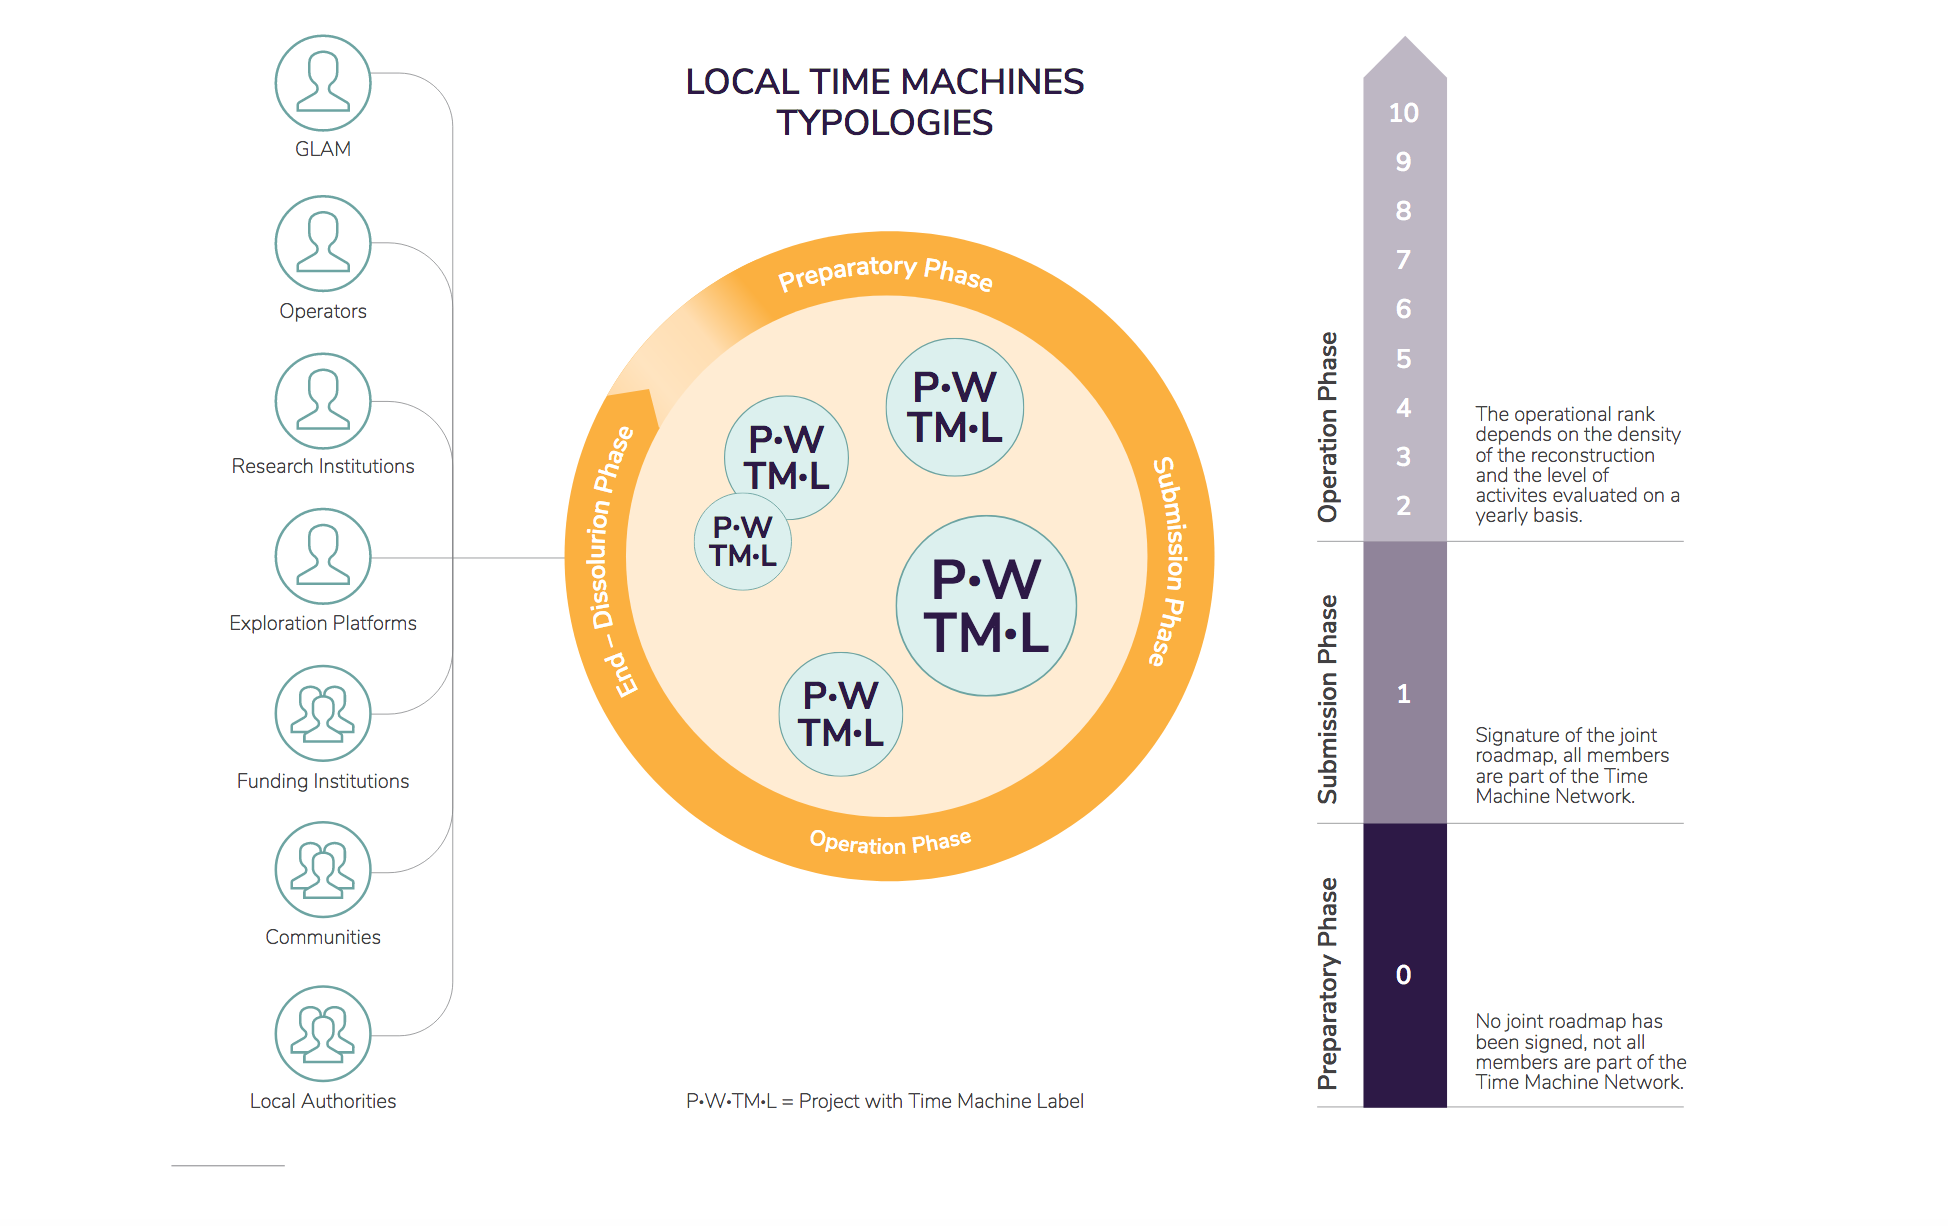
\includegraphics[angle=90, scale=0.7]{ltm.jpg}
\caption{Local Time Machines, document de travail \textit{© Copyright 2019 Time Machine}}
\end{figure}


\section{Rédaction de la feuille de route}

L'élaboration de la feuille de route s'est très vite révélée une tâche ambitieuse, puisqu'elle implique à la fois l'intégration des idées motrices à l'initiative Time Machine, telles que pensées par le \gls{dhlab}, dans le contexte de la recherche en humanités numériques, et la prise en compte des envies et attentes des différents partenaires. Rédigée à destination d'un réviseur mandaté par l'\gls{ue} et dans le but d'obtenir un financement, ce document doit à la fois faire rêver et concrétiser les idées de tous. 

Nous nous sommes vite trouvée confrontée à la réalité que derrière le nom du projet et la quête commune visant à proposer un \gls{graph} du passé, se cachaient autant de définitions que de membres du réseau. Notre travail de stagiaire a consisté en un difficile exercice de transcription de tous ces intérêts parfois divergents, parfois audacieux, vers une feuille de route commune, servant de base au futur cadre des opérations, mais suffisamment flexible et vaste pour intégrer les inévitables changements induits par sa longue durée et son financement des plus incertains. Mener à bien cette mission nous a poussée à comprendre très précisément les différents composants du futur réseau Time Machine, qu'ils soient d'ordre technique ou opérationnel. Le projet étant prévu pour se déployer sur dix ans, la feuille de route reste à un niveau relativement macro, puisqu'il est difficile de prévoir certains choix techniques ou stratégiques avant que l'infrastructure, le financement et la gouvernance ne soit eux-mêmes clarifiés.

Au début de notre stage, le projet en est à ses prémisses, tout reste à définir et les nombreuses questions que nous nous posons ne font que s'ajouter à la longue liste de celles auxquelles nous devons proposer une réponse, et celles qui sont posées par les membres du comité exécutif. Le temps n'est d'ailleurs pas aux palabres et à la réflexion, puisque l'échéance du rendu intervient tôt, nous n'avons malheureusement pas eu l'opportunité de mener l'intégralité du travail réflexif présenté dans ce mémoire avant le rendu de la feuille de route. Ce travail de recherche nous a d'ailleurs permis de remarquer certains manques qui seront signalés.

Notre méthodologie de travail s'est construite autour des éléments et des enjeux figurant dans la première proposition du projet faite à l'\gls{ue}, complétée par nos discussions avec les membres du consortium, du comité exécutif, les équipes du \gls{dhlab} et notre maître de stage. 

Travaillant au sein d'un environnement ouvert où chaque membre peut suivre la construction des idées de manière transparente, nous avons également bénéficié de remarques ciblées émanant de certains spécialistes partenaires du consortium.
%===ajouter une mention de où accéder à la roadmpa
Les premières semaines de notre stage ont consisté en un grand travail de définition, afin de proposer un socle commun construit autour d'une clarification du contexte des différents éléments du projet, sur lequel chaque \gls{wp} ou \textit{PILLAR} peut venir appuyer ses idées. Ce travail a conduit à l'élaboration de différents graphiques et documents, qui trouvent une version plus synthétisée dans la deuxième partie de la feuille de route, \textit{Pillar 2 Key concepts}. 

Nous avons également été confrontée à la difficulté que chacun des trois premiers \textit{PILLAR}s, bien que planifiés pour être écrits en parallèle, était destiné à influencer les choix des autres. Veiller à articuler ces propositions pour garantir une harmonisation des processus (entre les pistes de recherche identifiées dans le \textit{PILLAR 1} et les impacts envisagés par le \textit{PILLAR 3}) a impliqué des ajustements jusqu'aux derniers jours avant le rendu. Le détail de ces interactions figure également dans la deuxième partie de la feuille de route, \textit{Interaction of pillar 2 with pillars 1 and 3}. 

De manière générale, la construction de la feuille de route a nécessité une grande flexibilité, et de nombreuses versions ont vu le jour avant d'aboutir à celle introduite dans ce mémoire et disponible en annexe\footnote{La version soumise à l'\gls{ue} fait quelque 60 pages et est écrite en anglais. Vous pouvez la consulter sur la clé USB accompagnant ce mémoire.} Écrit à plusieurs mains, ce document, à la hauteur des projets de numérisation, est complexe, et chaque choix pourrait être analysé. 

Pour ne pas alourdir inutilement ce rendu et rester dans le cadre de notre problématique, nous ciblons notre présentation sur les réponses apportées par Time Machine aux enjeux de la numérisation. Bien que ces derniers ne soient pas décrits ainsi dans la feuille de route, les différentes solutions développées dans la partie trois \textit{Research and Innovation Plan}, complétés des éléments proposés par les autres \textit{PILLARs} et \gls{wp}s contribuent à y répondre et offrent un aperçu cohérent de notre expérience de stagiaire. 

La feuille de route figure sur la clé USB accompagnant ce mémoire.

\begin{figure}[ht]% force à placer l'image au sein de notre balise figure
%\centering
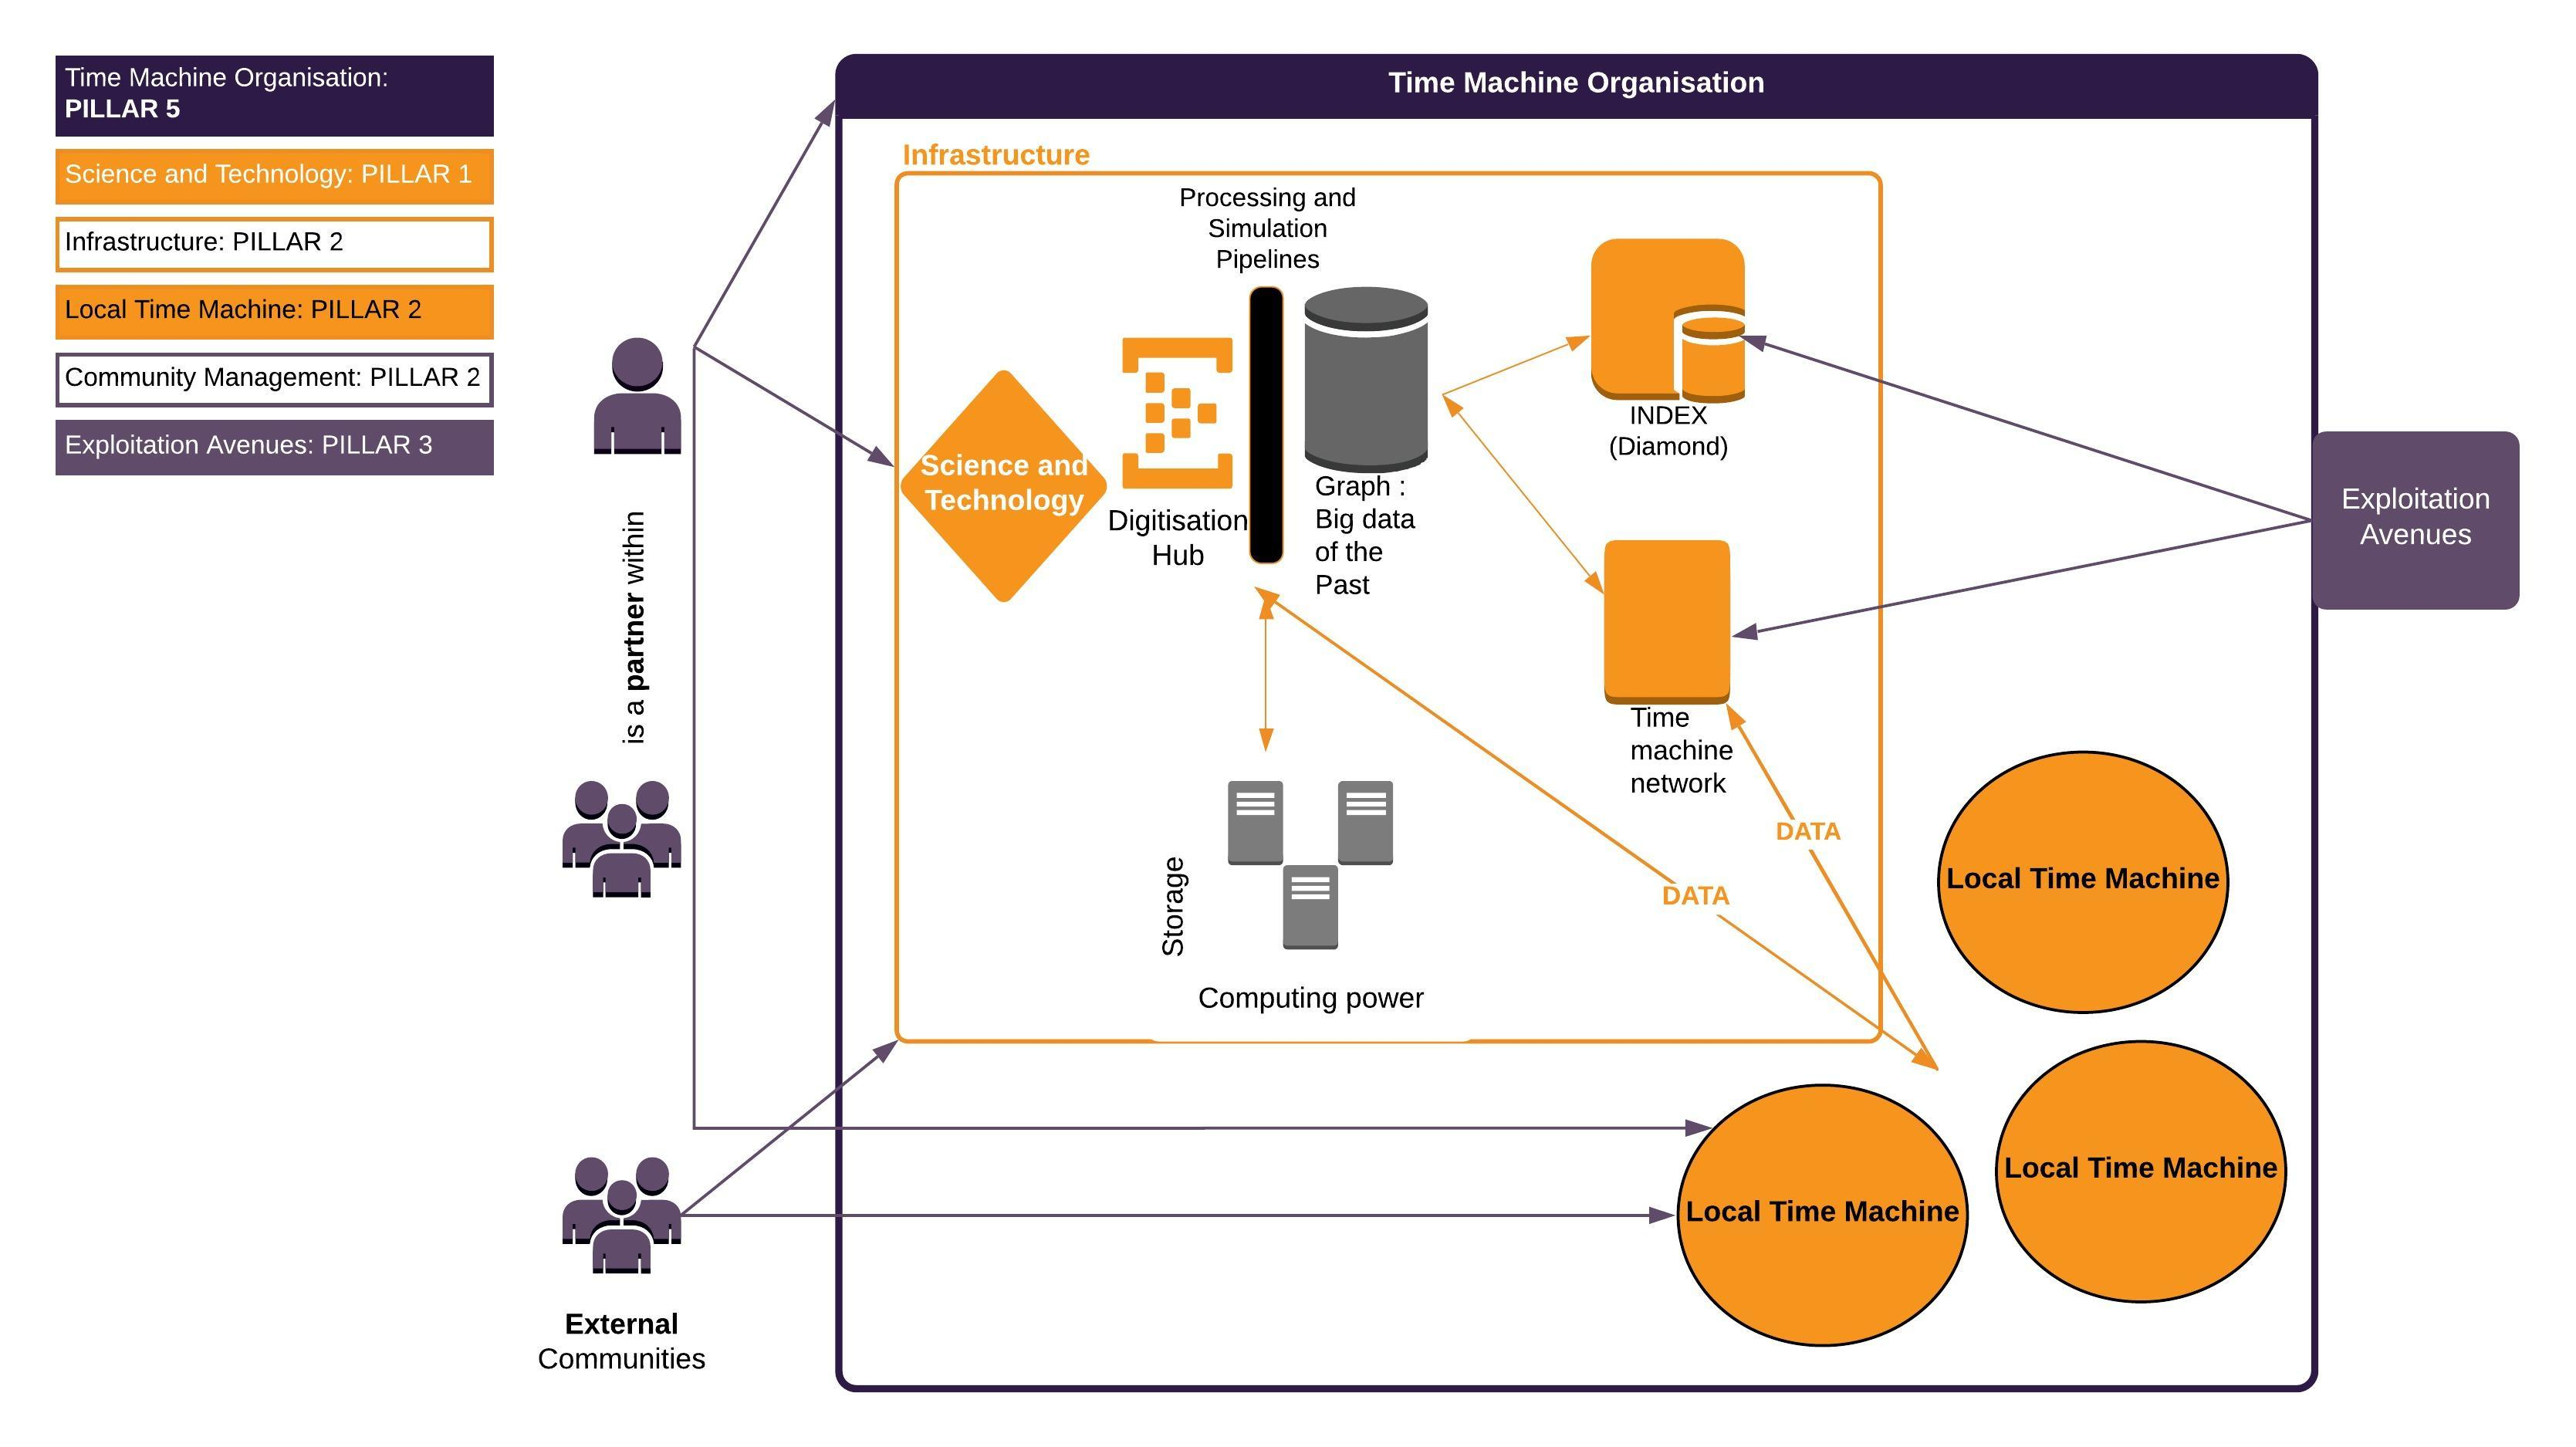
\includegraphics[angle=90, scale=0.9]{tmo.jpeg}
\caption{Les différents composants de la \textit{Time Machine Organisation}, document de travail}
\end{figure}

%==== REPONSES APPORTEES PAR TM AUX ENJEUX DE LA NUMERISATION
\chapter{Quelles réponses aux enjeux de la numérisation ?}

Le projet Time Machine étant encore dans un processus de définition, nous ne pouvons garantir que les propositions énoncées ci-après seront réellement implémentées après la période du \gls{csa}. Toutefois, elles reflètent les premières hypothèses et volontés organisationnelles, qui seront amenées à se concrétiser plus précisément au fil de l'avancement du projet.

\section {Amener différents acteurs à collaborer}
Time Machine est par essence un projet collaboratif qui vise à agréger les données de différentes institutions culturelles et patrimoniales.

Né d'une association de 33 institutions, le consortium compte désormais plus de 300 membres. Pour parvenir à co-construire ce projet, la collaboration est centrale à différents niveaux : entre les  partenaires appelés à concevoir l'organisation du projet et à partager des ressources ; entre le projet et les instances extérieures qu'elles soient politiques, académiques, privées, publiques ; entre le projet et le grand public. Afin de préserver ces relations, différentes démarches ont été entreprises et le déploiement des solutions contenues dans la feuille de route devront contribuer à préserver le futur de cette coopération. 

Conscients de l'importante de la collaboration pour une initiative de cette envergure et par conviction du pouvoir de l'intelligence collective, la collaboration sera intégrée aux futures valeurs du projet. Différents moyens seront mis en place afin de promouvoir l'existence d'espaces d'échanges et encourager un décloisonnement des activités au profit d'une logique de groupe. Un système de label sera par exemple développé afin d'encourager les différents projets composant Time Machine à favoriser cette pratique (des moyens qualitatifs serviront à l'évaluer).

Afin de favoriser l'acceptation, le développement et la mise à jour des futurs standards du réseau, un processus inspiré de celui utilisé pour définir les standards d'internet sera adopté : \gls{rfc}\footnote{Pour en savoir plus : \url{https://en.wikipedia.org/wiki/Request_for_Comments}}. Ce système consiste en la publication en ligne de propositions, dont les thématiques, voir les pistes de réponses, ont d'abord été définies par un comité d'édition en fonction des besoins du projet. Publiées de manière transparentes, elles sont soumises à la validation et aux critiques de la communauté, et ne sont implémentées que lorsque le consensus est atteint. La feuille de route contient de nombreuses propositions de \gls{rfc}s visant à mettre en place l'infrastructure et les opérations.

Le projet s'inscrivant dans une démarche de transparence, les composants techniques, ainsi que toute la documentation du projet seront accessibles sous licences \textit{\gls{cc}}, favorisant leurs réutilisations et le développement de nouveaux services. Le partage des connaissances et les développements technologiques font partie des objectifs du projet, qui s'inscrit dans la démarche d'\gls{os}.

Partenaire de grand réseaux culturels et patrimoniaux (à l'instar d'Europeana), Time Machine s'attachera à mettre en place des moyens dédiés à favoriser synergies et interactions entre ces différents acteurs, favorisant les échanges de bonnes pratiques et contribuant à l'accroissement des activités de ces réseaux et le développement d'outils communs. 

Les communautés de bénévoles spécialistes ou amatrices seront invitées à prendre une part active au sein des projets. Inscrivant Time Machine dans la mouvance des \gls{cs}.

Au sein de chaque Time Machine locale, un espace \textit{Smart Clusters}, servira à rassembler les potentiels futurs exploitants (industries culturelles et créatives, industries touristiques, instances politiques régionales etc.) et les partenaires de Time Machine, afin  d'impliquer les premiers dans la conception de projets, et assurer un ancrage de l'initiative locale au sein de son environnement et le déploiement d'une partie de ses activités autour de particularités et besoins ciblés.

\subsection{\textit{Complément} aux propositions de la feuille de route :}

Les données produites au sein des Time Machines locales étant destinées à alimenter le \gls{graph} du passé, ces dernières constituent un réseau de partenaires (\gls{agr}s) stratégiques, avec lesquels il faut particulièrement soigner la collaboration. La mise en place d'un forum similaire à celui d'Europeana ou \gls{dpla} favorisant les échanges devrait ainsi être considéré. La place des \gls{agr}s thématiques et régionaux déjà existants devra également être réfléchie.

\section {Financement et partenariats public-privé}

Un modèle de franchise sera mis en place, permettant aux différents partenaires de bénéficier de l'infrastructure de Time Machine, de formation et d'aide ciblée tout en contribuant à l'autonomie financière du projet. Ce dernier tiendra compte de différents critères et visera à clarifier les relations entre les Time Machines locales et la future gouvernance. 

Au-delà des partenariats financiers, le réseau mise sur la création de la \textit{Time Machine Infrastructure Alliance}, regroupant des partenaires extérieurs au projet mais intéressés à contribuer au développement de nouvelles technologies, et des philanthropes, qui seront invités à participer par des moyens plus concrets (puissance de calcul informatique, espace de stockage) à la durabilité du projet. 

Les différentes Time Machines locales seront à priori responsables du financement de leurs projets. 

Le consortium étant déjà composé d'un mélange entre partenaires publics et privés, cette spécificité sera conservée au sein de la future \textit{Time Machine Infrastructure Alliance}. Une attention particulière sera portée sur ces partenariats afin de garantir la mission de transparence et d'ouverture que s'est donné le projet. 

Il est possible que des institutions privées souhaitant bénéficier des outils de Time Machine puissent le faire, sans que leurs données soient utilisées pour alimenter le futur \gls{graph} de données du passé, ces dernières devront payer pour ce service en fonction d'une tarification préétablie.

Le financement servant à développer l'infrastructure du projet, n'est pas encore connu, mais le projet est en quête du soutien de l'\gls{ue}.


\section {Droit d'auteur}

Time Machine est amené à traiter deux typologies différentes de données : les privées et les publiques. Les données publiques (produites par des institutions publiques, ou données libres de droit) seront partagées sous licences \textit{\gls{cc}}, de préférence CC0. Les données privées (produites par des particuliers ou des institutions privées, données personnelles, ou données sous droit) seront protégées par des licences plus strictes et leur consultation pourra être sujette à certaines restrictions. Les données à caractère sensible (violentes ou illicites) publiées sous licence \textit{\gls{cc}}, seront également associées à des restrictions d'accès. 

Les différentes licences seront explicitées dans les métadonnées de chaque document. 

Les outils et processus permettant de faire face à ces typologies de données restent encore à déterminer.

\subsection{\textit{Complément} aux propositions de la feuille de route :}

La feuille de route ne mentionne pas précisément le besoin de créer et rendre visible un système de déclarations des droits d'usage pour améliorer l'accès aux ressources. Le traitement des \oe{}uvres orphelines ou hors commerce n'est pas non plus abordé alors que, suite aux exemples étudiés, nous préconiserions l'étude d'une stratégie de gestion des risques pour ces \oe{}uvres au statut légal incertain.

\section {Sortir des silos : enjeux techniques}

Europeana étant partenaire du réseau Time Machine, à priori son modèle de métadonnées (suivant les recommandations du modèle RDF) sera utilisé au sein du projet (pour les données non déduites) et l'architecture de Time Machine sera interopérable avec celle d'Europeana. Un modèle pour les données déduites sera élaboré, s'assurant de faire figurer explicitement les processus de création de ces informations dans leurs métadonnées. Une charte technique, contenant ces différentes spécifications devra être signée par tous les partenaires du réseau Time Machine. Time Machine prendra part aux réflexion menées sur les vocabulaires contrôlés \footnote{Rappel : Lexique servant à organiser les connaissances pour favoriser la recherche d'information} et les ontologies\footnote{\inquote{Rappel : Une ontologie est une façon de modéliser un domaine en identifiant les concepts y afférents et en les organisant les uns par rapport aux autres \cite{delestre_du_2017}.} }

En plus de la standardisation des métadonnées, Time Machine vise à normaliser les protocoles de numérisation, afin de garantir une qualité et une cohérence à travers tous les centres de son futur réseau européen de numérisation. 

Time Machine rendra obligatoire l'utilisation de \gls{iiif} pour les images, veillera au déploiement de différentes \gls{api}s et utilisera le protocole \gls{oai} .

\subsection{\textit{Complément} aux propositions de la feuille de route :}
La qualité de la numérisation devra être suffisamment élevée pour garantir un stockage sur le long-terme des données numérisées et les critères de cette qualité précisément étudiés.

En plus de l'usage de \gls{iiif}, \gls{oai} et autres \gls{api}s pour garantir l'interopérabilité, il serait judicieux d'offrir la possibilité aux futurs exploitants de disposer d'une exportation totale des bases de données (suivant l'exemple de \gls{dpla}).


\section {Sortir des silos : enjeux sur le contenu}

Mise en place d'un système de sélection des données (politique documentaire) s'inspirant des recommandations élaborées par \textit{The National Information Standards Organisation}\footnote{Pour en savoir plus : \url{https://www.niso.org/}.}, qui sont basées sur des critères liés aux besoins de recherche des institutions, unicité des documents, valeur du document etc. Bien qu'ayant vocation à numériser toutes les données du passé, il est probable que certains documents servant de base au développement de la future plateforme soient numérisés en premier (tels que les cadastres, journaux, cartes et plans). Time Machine ne se focalise pas sur un seul format de document et veut développer particulièrement la numérisation 3D.

\subsection{\textit{Complément} aux propositions de la feuille de route :}
Les manques hérités des politiques de numérisation des institutions partenaires, ou les différents biais qui peuvent être amenés à persister dans de nouvelles initiatives, devraient être étudiés et certains projets spécifiquement entrepris afin de rétablir l'équilibre.

Certaines mesures spécifiquement dédiées à faciliter la numérisation de données à partir du 20\up{e} siècle devraient être examinées afin de contribuer à sortir l'Europe de ce \inquote{trou noir} de l'information.


\section {Stockage sur le long-terme - préservation}

La préservation sur le long-terme des données de Time Machine sera prise en compte par le projet, afin que l'énorme travail de numérisation n'encourt pas le risque d'être perdu.

Time Machine propose des solutions de stockage à destination des petites institutions qui ne disposent pas d'espace suffisant sur leurs propres serveurs : les \textit{Time Machine Box}. Ces dernières existent à l'état de prototype et devront être améliorées (elles ne disposent pas encore de copie de sauvegarde).

Les données du projet seront stockées de manière partagée (à travers les ressources de la \textit{Time Machine Infrastructure Alliance}) sur des serveurs  spécialement conçus pour garantir leur préservation durable et prévenir tous risques d'accidents ou de dommages. 

Le poids des jeux de données et l'impact environnemental des serveurs faisant partie des préoccupations du projet, des solutions de stockage innovantes sont aussi envisagées.

\newpage
\section{Résumé des réponses de Time Machine aux enjeux de la numérisation}
\begin{table}[H]
\centering
\begin{tabular}{|l|l|}
\hline
\rowcolor[HTML]{2E1A46} 
{\color[HTML]{FFFFFF} \textbf{Enjeux}}                                                                                   & {\color[HTML]{FFFFFF} \textbf{Réponses de Time Machine}}                                                                                                                                                                                                                                                                                                                                                                                                                                           \\ \hline
{\color[HTML]{2E1A46} \textbf{\begin{tabular}[c]{@{}l@{}}Amener différents\\ acteurs à collaborer\end{tabular}}}         & \begin{tabular}[c]{@{}l@{}}Inscription de la collaboration dans les valeurs du projet et \\ création d'un système de labels. Utilisation des \textit{Request for}\\ \textit{Comments}. Publication et partage des différents développements \\ sous licence \textit{Creative Commons}. Échange avec les réseaux \\ partenaires. Intégration du grand public (sciences citoyennes).\\ Création de \textit{Smart Clusters}. Création d'un forum favorisant les\\ échanges entre les Time Machines locales et la gouvernance.\end{tabular} \\ \hline
{\color[HTML]{2E1A46} \textbf{\begin{tabular}[c]{@{}l@{}}Financement et \\ partenariats \\ public-privé\end{tabular}}} & \begin{tabular}[c]{@{}l@{}}Moyens financier assurés par les partenaires (redevance). \\ Soutien en nature possible à travers la \textit{Time Machine}\\ \textit{Infrastructure Alliance}. Vente de services à l'extérieur du \\ projet. Les Time Machines locales sont responsables du \\ financement de leurs projets. Partenariats public-privé déjà \\ existants et amenés à se développer. Recherche de financement \\ pour l'infrastructure auprès des instances européennes.\end{tabular}                   \\ \hline
{\color[HTML]{2E1A46} \textbf{Droit d'auteur}}                                                                           & \begin{tabular}[c]{@{}l@{}}Favorable à l'usage des licences \textit{Creative Commons}. \\ Restriction d'accès dans le cadre de données privées \\ ou sensibles. Métadonnées explicites. Déploiement \\ d'un système de déclaration des droits d'usage.\end{tabular}                                                                                                                                                                                                                                         \\ \hline
{\color[HTML]{2E1A46} \textbf{\begin{tabular}[c]{@{}l@{}}Sortir des silos : \\ enjeux techniques\end{tabular}}}          & \begin{tabular}[c]{@{}l@{}}Adoption du modèle de métadonnées développé par Europeana \\ et interopérabilité avec sa plateforme. Recours à des \\ vocabulaires contrôlés. Utilisation des différents outils tels que\\ APIs, IIIFs, OAI-PMH. Création de normes de qualité pour la \\ numérisation, amenées à se déployer à travers les futurs centres \\ de numérisation du réseau Time Machine.\end{tabular}                                                                                       \\ \hline
{\color[HTML]{2E1A46} \textbf{\begin{tabular}[c]{@{}l@{}}Sortir des silos : \\ enjeux sur le \\ contenu\end{tabular}}}   & \begin{tabular}[c]{@{}l@{}}Politique documentaire. Intégration des différentes typologies \\ de données et développement spécifique de la 3D. Analyse des\\ manques existants et actions ciblées pour y pallier.\end{tabular}                                                                                                                                                                                                                                                                        \\ \hline
{\color[HTML]{2E1A46} \textbf{\begin{tabular}[c]{@{}l@{}}Stockage sur le \\ long-terme - \\ préservation\end{tabular}}}  & \begin{tabular}[c]{@{}l@{}}Développement de solutions de stockage pour les petites\\ institutions. Le stockage des données sur le long-terme est\\ essentiel. Les données seront stockées pour être préservées \\sur les serveurs de la \textit{Time Machine Infrastructure Alliance}.\end{tabular}                                                                                              \\ \hline
\end{tabular}                                                                                        
\caption{Résumé des réponses de Time Machine aux enjeux de la numérisation}
\end{table}
\newpage



%====== LES INNOVATIONS DU PROJET TIME MACHINE
\chapter{Les innovations du projet}

En quoi Time Machine représente une solution innovante par rapport à d'autres initiatives de numérisation de masse ? Nous vous proposons un retour sur certaines ambitions du projet, qui, selon nous, contribuent à sa popularité toujours croissante parmi les institutions européennes.

\section {Mélanger les acteurs}

Une des forces de Time Machine, est d'avoir cherché à fédérer dès le départ en-dehors du cercle des institutions culturelles et patrimoniales. Représentatif des recherches conduites en humanités numériques, qui favorisent le mélange des pratiques, Time Machine réunit : le monde politique ; les industries créatives et touristiques ; les scientifiques de tous horizons ;  les réseaux et infrastructures existants ;  et le grand public. Tous ces acteurs sont invités à la création d'un projet commun, s'affranchissant des barrières et n'ayant pas crainte d'inviter les futurs exploitants à participer à la création de l'infrastructure.

S'offrant comme un objet d'étude malléable, le projet nourrit une ambition suffisamment grande (la numérisation du passé européen sous toutes ces formes), pour que chacun puisse envisager d'en bénéficier. 

L'élargissement des différentes typologies de partenariats est pris en compte par tous les groupes de travail du projet, qui veillent à demeurer les plus inclusifs possibles.


\section {Innovations technologiques }

Porté par l'\gls{epfl} dont la renommée scientifique n'est plus à démontrer, Time Machine promet d'être à la pointe de la recherche en \gls{ia}, mais également de contribuer à l'émergence et la démocratisation de nouvelles technologies, permettant à ses partenaires publics et privés d'en bénéficier. Rapide retour sur certaines de ces ambitions technologiques :

\begin{enumerate}
\item \textbf{Données enrichies et données déduites}

L'automatisation des processus d'extraction des informations contenues dans les documents numérisés constitue le premier développement technologique, permettant la construction du \gls{graph} de données du passé : le \textit{\gls{bigd}} du passé.

Les données numérisées sont ensuite complétées de données déduites à l'aide de trois moteurs de simulation : \textit{4D Simulation Engine}\footnote{Ce moteur permet de simuler tous les présents et passés possibles liés à une donnée numérisée, prenant compte du temps et de l'espace.}, \textit{Universal Representation Engine}\footnote{Permet la reconstitution d'espaces ou éléments physiques en fonction d'informations issues dans les données (textes, images, vidéos, 3D). Ce moteur est capable de reconstruire un bâtiment en se basant uniquement sur sa description, son origine géographique et son âge.}, \textit{Large-scale Inference Engine}\footnote{Permet de déduire des informations en reliant toutes les données de la base, ce moteur d'inférence permet de corroborer les informations déduites par le \textit{4D Simulation Engine}}. Ainsi les technologies de l'\gls{ia} permettront aux données du passé d'acquérir le même poids que les données de notre présent numérique. 

L'introduction de ces données \inquote{déduites} et toutes les transformations technologiques qui en découlent constituent un des changements majeurs apporté par Time Machine.


\begin{figure}[H]% force à placer l'image au sein de notre balise figure
%\centering
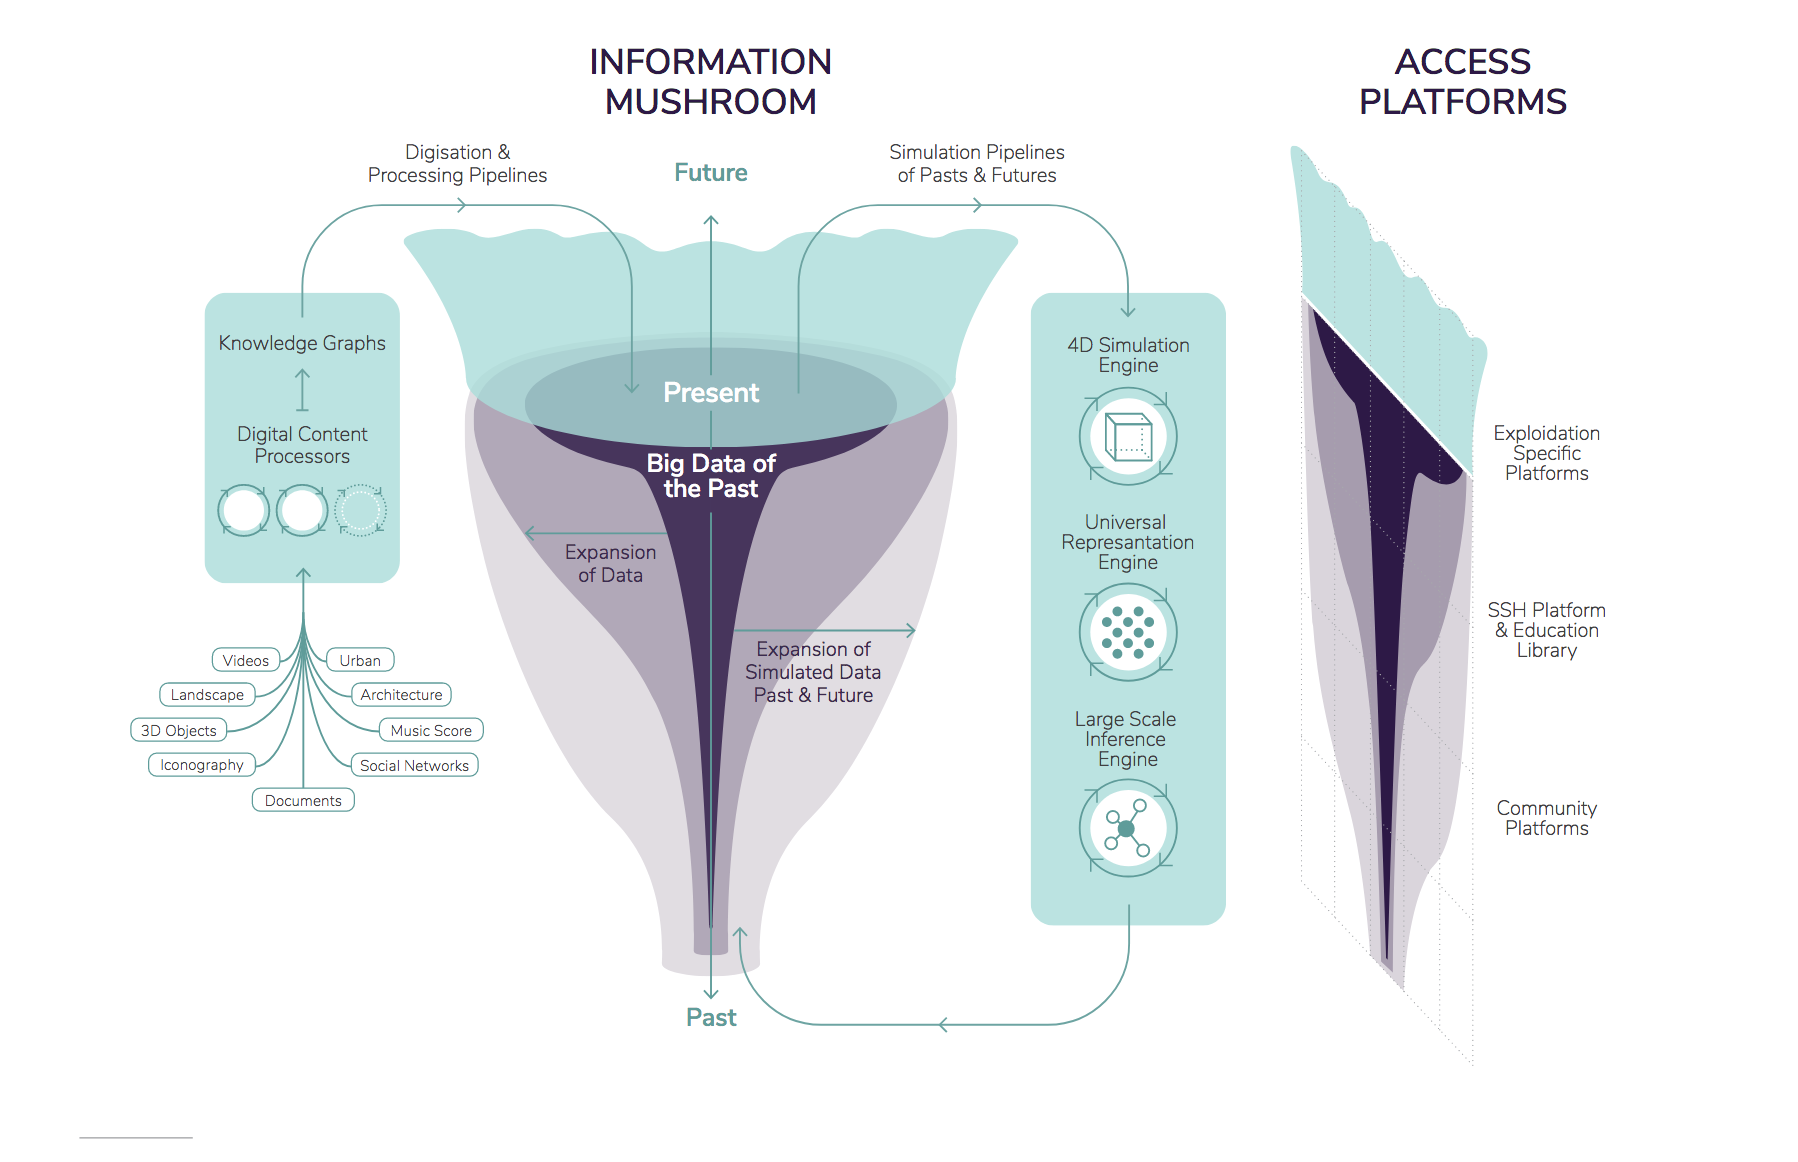
\includegraphics[scale=0.5]{simulation.jpg}
\caption{Représentation schématique des processeurs de contenus et des moteurs d'inférence \textit{© Copyright 2019 Time Machine}}
\end{figure}
\newpage
\item \textbf{Le facteur temps}

En ajoutant la temporalité aux outils de découverte traditionnellement déployés par les \gls{glam}s, Time Machine enrichira l'expérience utilisateur. Son moteur de recherche diachronique ouvrant de nouvelles perspectives de recherches et de valorisation des collections.

\item \textbf{3D et photogrammétrie}

Le \gls{dhlab} s'est spécialisé ces dernières années dans la reconstruction 3D du patrimoine. La \gls{photo} sera au centre des activités de la future initiative qui ne résume pas l'acte de numérisation du patrimoine aux objets 2D, mais promet de mettre l'accent sur la numérisation du patrimoine bâti et des collections muséales.

 Au même titre que Time Machine vise à organiser des centres de numérisation à travers l'Europe afin d'harmoniser les coûts et assurer un certain niveau de qualité, la photogrammétrie bénéficiera de son réseau de spécialistes européens.

\item \textbf{Archivage dans l'ADN}

Les données 3D sont très lourdes et l'ampleur du projet est telle, que de nouvelles solutions de stockage doivent être trouvées afin de permettre une préservation et une consultation de qualité. 

Le projet travaille avec différents partenaires actifs dans cette thématique, dont les propositions futuristes influenceront probablement notre monde de données de demain. L'archivage de données dans l'ADN fait partie de ces technologies prometteuses, permettant de stocker de manière stable et durable des informations, tout en minimisant l'impact écologique alloué à leur préservation. 

\item \textbf{Outils de numérisation}

La marché de la numérisation est encore dans une phase de construction, de nouvelles technologies seront amenées à améliorer les performances obtenues et à s'adapter à la fragilité de certaines typologies de documents. La tomographie\footcite{arte_tomography_nodate} constitue un outil des plus prometteurs, permettant de numériser un objet sans l'ouvrir et d'y déceler des particularités (liées aux fibres du papier etc.) jusqu'alors non visibles par une numérisation plus traditionnelle. Similaire à une radiographie, l'outil est sensible au taux de fer présent dans l'encre des manuscrits et permet d'obtenir des images en coupe de l'intégralité d'un volume. Time Machine promet de contribuer à la recherche sur ces nouveaux outils, et à leurs déploiements. 

\end{enumerate}

%====== RISQUES ET OPPORTUNITES POUR LE PROJET TIME MACHINE

\chapter{Risques et opportunités}

Au-delà des réponses aux enjeux de la numérisation, Time Machine doit faire face à certains risques et opportunités qui découlent de son contexte de création, mais sont aussi induits par les évolutions technologiques et les nouveaux services que le projet se propose de déployer.

\section {Plateforme, usages et accessibilité}

La masse des documents numérisés permet à la fois des recherches orientées, mais offre aussi de nouvelles méthodes de découvertes \inquote{\textit{[...]across genres and disciplines, as well as across institutional and national borders}.\footcite[p.123]{thylstrup_politics_2018}}. 

Au-delà de l'objectif de création de ce corpus de données, se pose la question de son accessibilité. Comment s'assurer que le travail mis en place par Time Machine puisse convenir aux usages des futurs utilisateurs ? Les nouvelles générations semblent peu enclines à la lecture, mais sont entraînées à la communication interactive\footcite{dufrene_numerisation_2013}, seront-elles dès lors à même de s'approprier le contenu et les interfaces de Time Machine ? Comment ne pas se retrouver dépassé par cette masse de données, pour mieux les présenter et les trier ?\footcite{xie_discover_2016}. Avec la numérisation de masse, la capacité humaine de \gls{cur} de ces collections numériques croissantes, semble dépassée. Les capacités cognitives des citoyens ordinaires et la puissance informatique sont de plus en plus sollicitées pour trouver du sens à cette accumulation de données\footcite{thylstrup_politics_2018}. Les fournisseurs de contenu ne peuvent plus se permettre de choisir un outil parmi d'autres, mais se doivent de construire avec tous les standards existants (\gls{api}, \gls{oai}, \gls{rdf} etc.)  pour s'assurer de délivrer leurs données aux plus larges audiences\footcite{dunning_digitising_2009}.

Le projet, à l'instar des précédentes initiatives, propose de réfléchir à de nouvelles formes d'outils de découvertes, promettant de nouvelles expériences aux utilisateurs. \inquote{\textit{An important question for builders of mass digitization projects has therefore been how to build visual and semantic infrastructure that offer the user a sense of meaningful direction as well as a desire to keep browsing.}\footcite[p.110]{thylstrup_politics_2018}}

\subsection{Franchir les barrières territoriales}

S'adressant à une communauté européenne, Time Machine doit être capable de gérer plusieurs langues. Ses utilisateurs souhaiteront pouvoir filtrer les résultats en fonction du langage et effectuer des recherches dans leurs propres idiomes\footcite{xie_discover_2016}. Le déploiement de solutions techniques devra tenir compte des particularités culturelles propres à chaque région et permettre une méthode de partage des données qui traduise automatiquement une requête dans toutes les langues et adresse des résultats provenant de chaque communauté linguistique\footcite{diekema_multilinguality_2012}.

La future plateforme du projet devra veiller à ne pas cloisonner ces résultats par le déploiement de normes occidentales qui préviendraient l'usage des produits à l'extérieur de sa propre communauté\footcite{jones_public_2017}.

\subsection{Être mobile}

La majeure partie du trafic d'Europeana étant générée par des mobiles, et étant donné l'évolution des pratiques et usages, le projet devra développer au plus tôt une telle interface\footcite{xie_discover_2016}\footnote{L'interface mobile de \textit{Diamond} est en cours de développement.}.

\subsection{Favoriser la cocréation}

Pour s'assurer de l'adéquation de la plateforme avec les pratiques des différentes communautés et garantir que ce projet, tourné vers différents publics, ne vienne pas à fonctionner comme la vitrine d'un projet de recherche mené par une communauté professionnelle\footcite{moatti_bibliotheque_2012}, Time Machine se doit de questionner les méthodes de développement traditionnelles et impliquer les usagers dès le début du projet, afin de proposer des services à même de satisfaire leurs besoins interactionnels \footcite[p.7]{dunning_digitising_2009}.

De nombreuses études (instaurées dès la fin des années 1990), ont cherché à comprendre pourquoi les ressources mises en place dans le contexte des humanités numériques n'étaient que peu utilisées par les chercheurs. Ces dernières ont conclu que leurs pratiques ne correspondaient que peu aux recherches empiriques, qui s'intègrent difficilement dans leurs routines de travail. De plus, les usagers semblent se désintéresser rapidement des outils numériques s'ils ne parviennent pas à accéder dès le départ à une information pertinente.\footcite{warwick_digital_2012}\footcite{warwick_studying_2012}. 

Les outils mis en place alors ne s'intéressaient pas du tout aux besoins et usages de leurs utilisateurs, qui étaient considérés comme incapables de comprendre les enjeux du numérique et dès lors de proposer leurs avis

Pour pallier à ce manque d'intérêt et d'adoption des données numériques par les chercheurs en humanités, il faut penser la création des plateformes dans la continuité des pratiques des communautés (ce qui signifie les étudier au préalable et les impliquer dans le processus de création) tout en offrant de nouveaux avantages. \inquote{\textit{If digital resources fit well with what they [users] want to do with them, users will adopt them.\footcite[p.18]{warwick_studying_2012}}}. \inquote{La plateforme fournit une infrastructure ouverte et participative pour des interactions créatrices de valeurs entre des producteurs et des consommateurs externes, dans le cadre des conditions de gouvernance définies par celles-ci.\footcite[p.100]{battu_histoire_2018}}

Les pratiques ne vont pas évoluer d'un coup, il faudra du temps pour que les communautés scientifiques adoptent véritablement ces nouveaux outils. Elles tendent toutefois à évoluer, poussant par exemple les historiens à s'adapter aux nouvelles méthodes d'analyse mises à leur disposition et à développer leurs outils de travail, les faisant prendre conscience de la nécessité de s'impliquer dans les processus de création de ces nouvelles ressources informationnelles. \inquote{If historians do not develop their tools themselves and embrace the goals of digital humanities, they are in danger of having method forced on them that are not compatible with their practice\footcite[p.25]{clavert_histoire_2013}.}

Les données doivent être mises à jour régulièrement, si les utilisateurs ont le sentiment que ces dernières sont dépassées ou datées, ils auront encore plus de difficultés à se les approprier. Leur préservation sur le long-terme doit aussi être garantie, car la recherche scientifique implique de pouvoir réutiliser des jeux de données pour comparer les résultats obtenus. La révolution numérique a instauré le doute concernant la durabilité et la reproductibilité de ces ressources\footcite{clavert_histoire_2013}. Si ces critères de mise à jour et de préservation ne sont pas respectés, il ne sert probablement à rien d'investir dans la création du projet. \inquote{\textit{This is a waste of the (probably) very large amount of money that was spent on its creation. Institutions have only recently begun to develop strategies to deal with this problem.\footcite[p.14]{warwick_studying_2012}}} La pauvreté des informations constitue également une menace, si les jeux de données sont construits uniquement pour un contexte précis, ils ne sauront être utilisés pour d'autres usages. Il faut garantir leur accessibilité intellectuelle afin de prévenir toute mauvaise compréhension des informations\footcite[p.67]{clavert_histoire_2013}.

Au-delà du public scientifique, les voix des communautés et des individus issues du \inquote{grand public} peinent également à être entendues au sein des projets de numérisation de masse \footcite{thelle_persuasive_2011}. La plateforme visant à s'adresser à la plus vaste audience possible, les publics empêchés doivent également être invités à participer au développement des futures interfaces.

Certains auteurs appellent à la construction d'une cyberinfrastructure au service de l'histoire, qui sera coconstruite avec les chercheurs en humanités et s'appuiera sur l'héritage des précédentes initiatives de numérisation, afin d'éviter que le savoir universel demeure détenu, de façon monopolistique, par quelques compagnies privées et puisse bénéficier à tous. Cette cyberinfrastructure devra permettre la création de nouveaux standards capables d'inviter les utilisateurs à chercher de l'information et à la transformer en connaissance\footcite{clavert_histoire_2013}. 

Il semble que Time Machine soit dès lors bien placé pour répondre à ce souhait, pour autant qu'il soit capable d'intégrer ses différents publics-cibles dans ses processus de création et d'inviter le grand-public à se positionner aux côtés de la communauté scientifique.


\subsection{Moteur de recherche ou plateforme de découverte ?}

Time Machine doit se positionner face aux géants de l'information déjà existants, qui ne travaillent pas uniquement à la création de corpus mais à l'indexation du web dans son ensemble. Entre site internet et moteur de recherche, le débat est encore vif et n'apporte que peu de réponse. Certains argumentent qu'un site ne saura rivaliser avec un moteur capable d'en indexer des millions\footcite{moatti_bibliotheque_2012} lorsque d'autres s'interrogent sur la valeur en terme de diffusion, de fonds numérisés ou de moteurs de recherche\footcite{dufrene_numerisation_2013}. Il semble qu'à ce jour, la seule méthode consiste en une forme de collaboration avec ces autres géants, et au déploiement de méthodologie de référencement\footnote{Terme rassemblant toutes les actions visant à améliorer la visibilité d'un site web dans les résultats naturels d'un moteur de recherche. Ces actions impliquent notamment le déploiement de schéma de métadonnées spécifiques, l'usage de mots-clés etc.}, que nous n'aborderons pas plus en détails dans ce présent mémoire.

\section {Crowdsourcing et sciences citoyennes}

Avec l'avènement du web social, de nouveaux moyens de création de ressources informationnelles ont vu le jour, sous la forme du \textit{crowdsourcing} d'abord, reflétant le transfert de processus de travail vers une main d'\oe{}uvre composée d'internautes, puis évoluant vers l'approche plus participative des \gls{cs}. Les entreprises de numérisation de masse et les \gls{glam}s, utilisent traditionnellement les compétences de ces communautés ou individus pour transcrire, corriger ou indexer une sélection de matériel\footcite{coutts_stepping_2017}. 

Le \textit{crowdsourcing} n'est toutefois pas apparu avec l'avénement du numérique, puisque déjà en 1859 la \textit{Philological Society} s'adressait aux citoyens afin de créer ce qui deviendra la première version du \textit{Oxford English Dictionary}\footcite{gupta_enriching_2017}.

De nombreux projets ont recours au \textit{crowdsourcing} pour la création des collections à numériser, invitant les individus à déposer leurs archives personnelles. Cette pratique tend à augmenter l'intérêt et la visibilité de ces initiatives, bien que suscitant des débats sur la qualité et la pertinence de ces nouveaux contenus\footcite{coutts_stepping_2017}. Ces communautés sont également appelées à collaborer dans le déroulement des activités de \gls{photo} liées à la numérisation 3D, qui offrent de nouvelles opportunités à forte valeur ajoutée \inquote{\textit{[...]which has particular intrinsic and instrumental value for themselves, and for their museums in their communities.\footcite[p.22]{chng_crowdsourcing_2019}}}, dans un contexte où les institutions n'ont souvent pas les moyens pour engager des équipes professionnelles \footcite{chng_crowdsourcing_2019}. Certains auteurs appellent à travailler avec les communautés d'expertise déjà existantes afin d'alléger les coûts engendrés par les recherches des détendeurs de droit des \oe{}uvres orphelines, favorisant leur numérisation et garantissant ainsi une marge d'erreur moins grande dans les résultats, puisque ces pratiques intègrent souvent des processus d'auto-vérification\footcite{stobo_i_2018}.

Si le \textit{crowdsourcing} peut prendre une grande variété de formes, en fonction des organisations et du contexte des projets, certains facteurs favorisent leur réussite : accessibilité des plateformes, coût, environnement de travail, ressources humaines etc.\footcite[p.27]{gupta_enriching_2017}. Les projets ayant recours au \textit{crowdsourcing} doivent être pensés dans la durée, puisqu'il est contreproductif de créer une communauté puis de la laisser tomber\footcite[p.15]{warwick_studying_2012}.

S'il faudra encore attendre quelques années pour bien comprendre l'articulation de ces \gls{cs} au sein des projets de numérisation, il est indiscutable qu'elles auront un rôle à jouer. Le modèle économique de Google semble basé sur une certaine idée du \textit{crowdsourcing} faisant appel à l'inventivité et l'intelligence collective du plus grand nombre, \inquote{[...]ces plateformes gratuites rebattent largement les cartes des règles commerciales et des frontières entre le marchand, le public, le commun et leurs différents domaines.\footcite[p.37]{dufrene_numerisation_2013}}. Certains y voient aussi le dernier rempart pour garantir l'accessibilité de toute la connaissance humaine et échapper aux logiques sélectives, dictées par le plébiscite des audiences légitimant certains contenus\footcite[p.107]{mattelart_histoire_2018} : 

\begin{quotation}
Seules des \inquote{sciences citoyennes} qui échappent à l'élitisme tout en se gardant de faire le jeu du populisme peuvent faire contrepoids au projet de société globale de l'information porté par les géants du numérique, leur culture du résultat et du retour sur investissement à court terme. C'est là une condition nécessaire à l'essor de nouveaux usages démocratiques du potentiel du réseau des réseaux.\footcite[p.110]{mattelart_histoire_2018}
\end{quotation}

Time Machine a déjà pris en compte ces communautés dans la création de la feuille de route, il s'agira pour le projet de définir quelle forme et quel rôle attribuer à ces \gls{cs}, garantissant à la fois la préservation d'une continuité démocratique, et porteuses de changement.

\section {Pour un savoir cohérent, égalitaire et éthique}

Au-delà des critères de sélection hérités des politiques documentaires des institutions, Time Machine a l'opportunité de contribuer à créer une connaissance humaine plus juste et égalitaire, qui ne reproduit pas forcément les inégalités hiérarchiques héritées de notre société humaine. Ce défi n'est pas des moindres, puisque jusqu'à présent les plateformes informationnelles ont au contraire servi à renforcer ces mécanismes.

\begin{quotation}
[\textit{Traduction}]
Ce que nous avons constaté dans la pratique, c'est que les plateformes numériques ont la capacité de produire davantage d'homogénéité plutôt que l'inverse, à reproduire les logiques hiérarchiques, inégalités et biais qui structuraient l'existence humaine dans la société avant l'avènement d'internet\footnote{\inquote{\textit{What we have seen in practice is that online platforms have the capacity to produce more homogeneity rather than less, to cultivate and reproduce the hierarchical logics, inequalities, and biases that structured human existence in the world before the internet.}} \cite[p.22]{kim_race_nodate}}.
\end{quotation}

Le monde occidental étant très représenté au sein des acteurs de la numérisation de masse, Time Machine devra porter une attention particulière à la création de liens entre des réseaux de normes et de traditions culturelles différents de son propre milieu, afin de permettre une représentation plus objective de la connaissance qui, elle, s'affranchit aisément des frontières (ce biais impacte également le déploiement d'outils spécifiques à la numérisation, et le développement des plateformes d'accès)\footcite{weiss_examining_2016}\footcite{jones_public_2017}. 

En tant que futur \gls{agr} des collections d'institutions diverses, Time Machine devra veiller à proposer des collections satisfaisantes pour les besoins d'une immense variété de publics. Trouver un équilibre entre la construction de la cohérence et l'exhaustivité à laquelle tend le projet sera l'un des défis de sa future politique documentaire.

De nombreuses questions éthiques sont également soulevées par les initiatives visant à numériser la connaissance universelle. Que doivent-elles faire concernant les objets aux contenus racistes, sexistes, appelant à la haine ou à la suprématie de certains peuples ?\footcite{weiss_examining_2016} Comment garantir que le projet est fidèle aux critères moraux européens ? Si Time Machine veut réussir là où les précédentes initiatives ont échoué, il s'agira d'apporter des réponses à ces questions incontournables et d'offrir davantage qu'une restriction d'accès, comme solution au caractère sensible de certaines données.
\newpage
\section {Résumé des risques et opportunités pour Time Machine}
\begin{table}[H]
\centering
\begin{tabular}{|l|l|}
\hline
\rowcolor[HTML]{2E1A46} 
{\color[HTML]{FFFFFF} \textbf{\begin{tabular}[c]{@{}l@{}}Risques et opportunités\\ pour Time Machine\end{tabular}}}         & {\color[HTML]{FFFFFF} \textbf{Résumé}}                                                                                                                                                                                                                                                                                                                                                                                                                                                                                                                                                                                                                                       \\ \hline
{\color[HTML]{2E1A46} \textbf{\begin{tabular}[c]{@{}l@{}}Plateforme, usages\\ et accessibilité\end{tabular}}}               & \begin{tabular}[c]{@{}l@{}}S'affranchir des barrières territoriales : multilinguisme\\ et prévention contre l'usage de pratiques "occidentales".\\ Être mobile.\\ Favoriser la cocréation : impliquer les futurs usagers dans le\\ développement d'une plateforme ouverte et participative, \\ favorisant des interactions créatrices de valeurs. Veiller aux\\ mises à jour et à l'accessibilité sur le long-terme. Intégrer\\ l'héritage des précédentes initiatives.\\ Moteur de recherche ou plateforme de découverte ? Trouver \\ un positionnement adéquat et déployer des techniques de \\ référencement.\end{tabular}                                                     \\ \hline
{\color[HTML]{2E1A46} \textbf{\begin{tabular}[c]{@{}l@{}}Crowdsourcing et\\ sciences \\ citoyennes\end{tabular}}}           & \begin{tabular}[c]{@{}l@{}}Utiliser les compétences des communautés pour transcrire,\\ corriger ou indexer les collections, sélectionner les documents, \\ participer à la numérisation 3D (photogrammétrie), rechercher \\ les détendeurs des droits d'\oe{}uvres orphelines.\\ Garantir sa réussite, par le développement de plateformes\\ accessibles, une prise en charge des coûts sur le long-terme, un \\ environnement de travail valorisant, des ressources humaines\\ dédiées.\\ Définir le rôle du volontaire entre gardien de la démocratie et de \\ l'accessibilité et briseur des frontières entre marchand, public et\\ commun.\end{tabular} \\ \hline
{\color[HTML]{2E1A46} \textbf{\begin{tabular}[c]{@{}l@{}}Pour un savoir \\ cohérent, égalitaire et\\ éthique\end{tabular}}} & \begin{tabular}[c]{@{}l@{}}Ne pas reproduire les inégalités hiérarchiques de notre société.\\ Créer des passerelles au-delà du monde occidental pour \\ permettre une représentation nouvelle du savoir.\\ Trouver un équilibre entre construction de la cohérence et quête\\ d'exhaustivité.\\ Adresser les questions éthiques posées par la création des \\ collections et les objectifs du projet.\end{tabular}                                                                                                                                                                                                                                                             \\ \hline
\end{tabular}
\caption {Résumé des risques et opportunités pour Time Machine}
\end{table}

%====== POURQUOI NUMERISER EN MASSE

\chapter{\textit{Pourquoi} numériser en masse ? }

Nous avons essayé à travers ce mémoire, de montrer la complexité des entreprises de numérisation de masse. Du passage à l'échelle des premières entreprises de numérisation jusqu'à l'avènement des \gls{bigd}, ces projets ont franchi les portes de leurs institutions pour se mêler à l'agenda politique et prendre une part active dans la définition des standards du web. Porteurs de nombreux intérêts mélangeant biens communs et usages commerciaux, ils semblent rassembler sous la même bannière, des idées à priori opposées et des acteurs issus du monde public et du monde privé. Leurs poids financiers et les débats légaux qu'ils suscitent les poussent à inventer de nouvelles formes de partenariats et confrontent la sphère politique aux usages du numérique. Time Machine, bien que né dans un centre de recherche en humanités digitales, fédère au-delà de son milieu académique, s'affranchissant des barrières nationales, et à travers ses ambitions de recherche et de valorisation, semble incarner les questionnements de tous sur notre société numérique. Le projet, comme ses précurseurs, ne se laisse pas résumer par une seule question. Dernière initiative de la lignée des projets de numérisation de masse, Time Machine entend préserver le passé tout en modifiant l'avenir.

Au-delà des aspects techniques et opérationnels liés à l'envergure de ces projets, il semble urgent de considérer les questions du \textit{pourquoi}, afin de mieux comprendre l'impact d'initiatives de telle ampleur sur l'organisation de notre société et les industries qui la composent. Les questions soulevées sont nombreuses et nous ne prétendrons pas pouvoir leur apporter à toutes un début de réflexion, nous avons préféré introduire ce débat à travers deux questions qui nous semblent peu abordées par la communauté scientifique dans le cadre de tels projets\footnote{Le temps que nous avons eu à disposition pour la rédaction du mémoire étant cependant limité, il est probable que de nombreuses publications n'aient pas été prises en compte dans notre revue de la littérature. Notre impression est dès lors subjective.} : la surveillance de masse et le positionnement de ces initiatives par rapport aux acteurs culturels et patrimoniaux plus traditionnels.

\section {Influence de masse}

Bien que les projets de numérisation de masse se construisent autour de l'objectif de rendre accessible le savoir en ligne, et que les complexités liées à la construction des infrastructures et les questions financières, politiques, éthiques et légales qui en découlent tendent à accaparer toute l'attention, une autre forme de connaissance est acquise de manière plus discrète. Elle est sans doute motivée par des intérêts divergents en fonction des acteurs de chaque initiative et justifiée par le souci de proposer une meilleure expérience aux utilisateurs ou obtenir de nouvelles formes de financement. Nos actes et pensées d'usagers sont néanmoins précieusement récoltés, nous livrant à la merci de nouvelles logiques économiques et régimes politiques : \inquote{\textit{[...]as we collect and connect, we are also ourselves collected and connected.}\footcite[p.138]{thylstrup_politics_2018}}. 
Si les défenseurs de l'innovation argumentent qu'il ne sert à rien de s'effrayer de l'impact de ces collectes de données, qui auraient moins d'effet que les spots publicitaires traditionnels accompagnant les campagnes politiques : \inquote{\textit{We freak out over the unsavory influence of social media on our politics, while TV's partisan influence on elections is far, far greater than Facebook's.}\footcite{kelly_ar_2019}}. Il semble important de nous rappeler que nous avons un rôle à jouer dans la définition éthique des projets de cette envergure.

Les projets de numérisation de masse ont de plus recours aux technologies dites persuasives pour développer l'interface de leurs plateformes\footnote{Les technologies persuasives sont conçues pour modifier les pratiques et comportements des usagers à travers la persuasion et l'influence sociale, sans utiliser la force. Elles s'incarnent souvent dans le graphisme des interfaces et sont motivées par la recherche du \inquote{moindre effort}. Par exemple un usager ayant appris à effectuer des recherches sur Google, sera d'autant plus enclin à utiliser la même méthode pour accéder aux ouvrages de \textit{Google Books}. \cite{thelle_persuasive_2011}}, ces technologies basées sur les principes du \inquote{moindre effort} contribuent à la mise en place de mécanismes de pouvoir invisibles, susceptibles d'influencer notre liberté d'opinion et la démocratie\footcite{thelle_persuasive_2011}. 

Le pouvoir de ces entreprises étant souvent le résultat d'un petit nombre de personnes qui décident pour toutes les autres\footcite{thylstrup_politics_2018}, ce sont néanmoins les utilisateurs finaux qui permettent à ce marché d'exister. Dès lors une prise de conscience de ces enjeux permettrait de rétablir un équilibre entre tous ces intérêts divergents, et contribuerait à garantir que l'emploi de ces technologies se fasse bien au service de la démocratie.


\section {Vers la création d'un nouvel acteur de l'information}

Nous nous sommes interrogée, en introduction de ce mémoire, sur la place occupée par ces projets au sein de la famille des institutions culturelles ayant pour mission de rendre la connaissance accessible à tous (\gls{glam}), puisque les initiatives de numérisation de masse sont d'abord et premièrement motivées par une mission similaire : celle de restituer au monde la connaissance, en s'assurant de son accessibilité dans notre société numérique, à travers la numérisation.

L'étude des différents enjeux de la numérisation et l'analyse d'autres initiatives témoignent que le succès de ces projets n'est pas seulement corrélé aux seules capacités des institutions culturelles et patrimoniales, mais implique un mélange d'acteurs issus du monde privé et du monde public répondant à des communautés de pratiques et à des politiques diverses, s'organisant au sein d'un réseau. L'infrastructure commune aux membres de ce réseau doit être par essence souple et flexible, capable de s'adapter à la diversité de ses partenaires, tout en définissant un certain nombre de standards et de routines permettant une convergence des pratiques. La mise en place de ces standards aboutit à des formes de politiques internes au réseau et contribuent à renforcer son pouvoir vis-à-vis des politiques extérieures. Le pouvoir du réseau se construisant souvent en même temps que le réseau lui-même : \inquote{\textit{through standardization, inventions become commonplace, novelties become mundane, and the local becomes universal.}\footcite[p.31]{thylstrup_politics_2018}}.

Le déploiement d'activités de numérisation de masse offre la perspective de création de nouvelles sources de revenus, attirant industries et entreprises privées au sein de leurs réseaux. Les entreprises culturelles étant depuis toujours empreintes de capitalisme, la numérisation de masse a de facto introduit une nouvelle forme de capitalisme imposée à notre mémoire culturelle : le capitalisme numérique\footcite{thylstrup_politics_2018}. 

Ces initiatives semblent, de plus, contribuer à inscrire les institutions patrimoniales et leurs usagers au sein d'une nouvelle constellation de pouvoir et de politiques : \inquote{\textit{[...] these infrapolitical imaginaries in fact show the complexity of mass digitization projects in their reinscription of users and cultural memory institutions in new constellations of power and politics.} \footcite[p.131]{thylstrup_politics_2018}}.

Plus que de simples plateformes de valorisation visant à rendre les données du passé accessibles, le déploiement de l'infrastructure des projets de numérisation de masse soulève de grandes questions concernant l'éthique, les politiques, le pouvoir et la protection des individus au sein de la sphère numérique. Issues de différents courants politiques, ces initiatives viennent bouleverser l'organisation existante du pouvoir.
\begin{quotation}
[\textit{Traduction}]
La luxuriante dimension des initiatives de numérisation de masse semble émerger des décombres de processus politiques perturbateurs et tumultueux, qui viennent violemment disloquer les frontières établies et les dynamiques de pouvoir, donnant naissance à de nouvelles formes qui doivent encore être interprétées. \footnote{\inquote{\textit{Rather, the productive dimensions of mass digitization emerge from the rubble of disruptive and turbulent political processes that violently dislocate established frontiers and power dynamics and give rise to new ones that are yet to be interpreted.\cite[p.137]{thylstrup_politics_2018}}}} 
\end{quotation}

Difficile en conséquent de considérer ces initiatives comme une simple évolution des activités conduites par les institutions culturelles et patrimoniales. Si ces projets tendent à bouleverser les règles établies et sont suffisamment puissants pour impacter les politiques et proposer une nouvelle forme d'économie, ils se doivent probablement d'être considérés en tant que nouvelle entité (ou acteur de l'information), dont les particularités et caractéristiques doivent encore être pleinement étudiées et comprises, afin de ne pas laisser ce pouvoir émergent se construire en-dehors des règles fondatrices de notre société.


